\documentclass[12pt, a4paper]{article}

\usepackage[utf8]{inputenc}
\usepackage[russian]{babel}
\parindent 0pt
\parskip 8pt
\usepackage{amsmath}
\usepackage{amssymb}
\usepackage{array}
\usepackage{floatrow}
\usepackage{float}
\usepackage[left=2.3cm, right=2.3cm, top=2.7cm, bottom=2.7cm, bindingoffset=0cm]{geometry}
\usepackage{hyperref}
\usepackage{graphicx}
\usepackage{multicol}
\usepackage{listings}
\usepackage{fancyhdr} 
\usepackage{extramarks}
\usepackage[usenames,dvipsnames]{color}
\usepackage{titlesec}
\usepackage{tikz}
\usepackage[T2A]{fontenc} 
\definecolor{grey}{RGB}{128,128,128}
\everymath{\displaystyle}

\title{Рабочий протокол и отчет по лабораторной работе № 5.04
\\ Определение постоянной Ридберга для атомного водорода
}

\author{Фадеев Артём }
\date{Апрель 2022}

\begin{document}

\maketitle
\section{Цель работы}

\begin{itemize}
    \item Получение численного значения постоянной Ридберга для атомного водорода из экспериментальных данных
    \item Сравнение с рассчитанной теоретически
\end{itemize}

\section{Объект исследования}

\begin{itemize}
    \item Атом водорода
\end{itemize}

\section{Рабочие формулы и исходные данные}

\begin{itemize}
    \item Длина волны:
    
    $\lambda = B \frac{n^2}{n^2 - 4}$
    \item Волновое число:
    
    $\tilde{v_0} = \frac{1}{\lambda}$
    \item Формула Бора:
    
    $E_n = -\frac{2 \pi^2 m e^4}{h} \cdot \frac{1}{n^2} = -hcR \frac{1}{n^2}$
    
    $R = \frac{2\pi^2 me^4}{ch^3}$(СГС), $R = \frac{me^4}{8ch^3{\epsilon_0}^2}$ (СИ)
    
    \item Серия Бальмера
    
    $\tilde{v_0} = R \cdot (\frac{1}{2^2} - \frac{1}{n^2})$
\end{itemize}

\section{Измерительные приборы}

\begin{itemize}
    \item Водородная трубка, ртутная лампа
    \item Монохроматор
    \item Источник питания ртутной лампы и водородной лампы
    \item Источник питания подсветки монохроматора
\end{itemize}

\section{Схема установки}

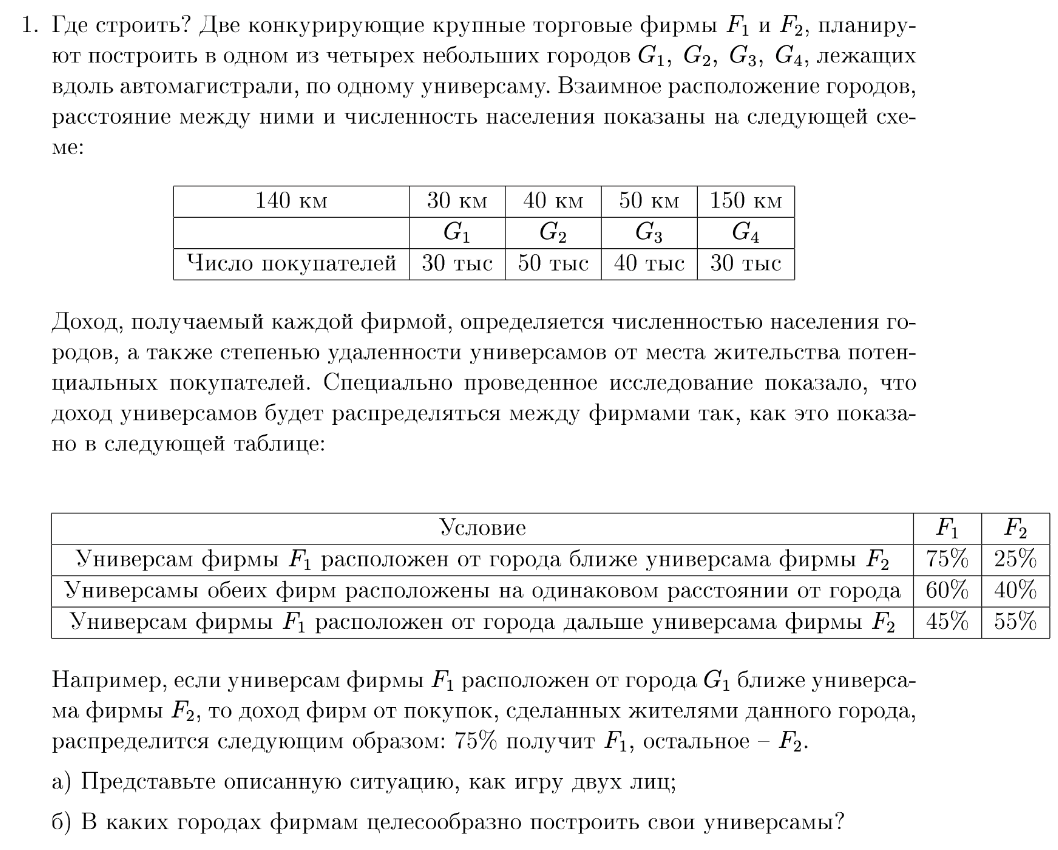
\includegraphics{1.png}

\section{Результаты прямых и косвенных измерений и их обработки}

Цвет линий в спектре ртути

\begin{tabular}{|c|c|c|}
     \hline & \lambda, um & \alpha, del\\
     \hline Красный & 690.7& 2537\\
     \hline Красный &  671.1 & 2515\\
     \hline Оранжевый & 623.4 & 2181 \\
     \hline Желтый & 579 & 2065 \\
     \hline Желтый & 576.9 & 2056 \\
     \hline Зеленый & 546 & 1866 \\
     \hline Голубой & 491.6 & 1450 \\
     \hline Сине-фиолетовый & 435.8 & 790 \\
     \hline Фиолетовый & 407.8 & 530 \\
     \hline Фиолетовый & 404.7 & 456 \\
     \hline
\end{tabular}

Цвет линий в спектре водорода

\begin{tabular}{|c|c|c|}
     \hline & \lambda, nm & \alpha, del \\
     \hline Красный & 643.592 & 2378 \\
     \hline Голубой & 485.461 & 1398 \\
     \hline Фиолетовый & 426.198 & 756 \\
     \hline
\end{tabular}

\begin{tabular}{|c|c|c|}
     \hline Цвет & $\tilde{v}$, nm & 1/n^2 \\
     \hline Красный & 1553779,413 & 0.108\\
     \hline Голубой & 2059897,705 & 0.062 \\
     \hline Фиолетовый & 2346327,294 & 0.036 \\
     \hline
\end{tabular}

\begin{tabular}{|c|c|c|}
     \hline Значение & R, m^{-1} & E, eV \\
     \hline Из угла наклона пряиой & 11000000 & -13.63 \\
     \hline Из ординаты точки пересечения & 10960000 & -13,571 \\
     \hline Теоретически & 10973731 & -13,592 \\
     \hline Погрешность, \% & 0,0571 & 0,0574 \\
     \hline
\end{tabular}

\section{Графики}

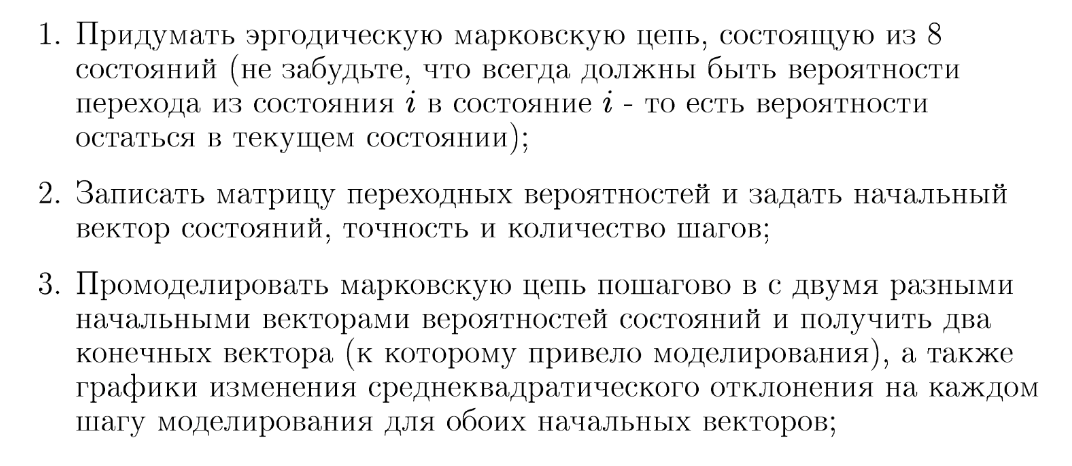
\includegraphics[scale=0.85]{2.png}

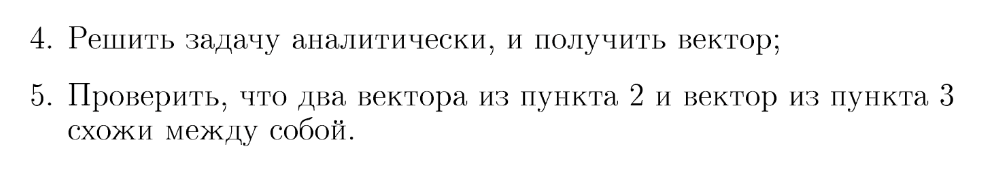
\includegraphics[scale=0.85]{3.png}


\section{Выводы и анализ работы}

\begin{itemize}
    \item В ходе выполнения работы была снята градуировочная кривая монохроматора, определены длины волн спектра водорода, рассчитаны соответствующие волновые числа и вычислено экспериментальное значение постоянной Ридберга, погрешность измерения которого составила 0,0571%
\end{itemize}
\end{document}